% !TEX root= ../main.tex
\section{Inconsistencies in graph theories}
\label{sec:Inconsistencies in graph theories}
In this section, we will prove the existence of non-binary-derivable inconsistencies from graphs.
We will first prove a lemma, then apply this lemma to an extended version of the graph from Figure~\ref{fig:double_open_door} to show that its inconsistency is not binary-derivable.

Let $G$ be a digraph with a source vertex (a vertex with no predecessors) $x$.
Let $A$ and $B$ be two disjoint subgraphs of $G$ such that $N(A) \subseteq A$ and $N(B) \subseteq B$ and such that $N^-(A) \setminus A = N^-(B) \setminus B = \{ x\}$.
In words, nothing points out of $A$ and $B$ and only $x$ points in.
Note that $x$ might have additional successors.\par
\begin{figure}[!h]
  \centering
  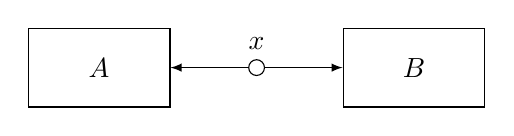
\begin{tikzpicture}
    [
    point/.style={circle,draw,inner sep=0pt,minimum size=2mm},
    collection/.style={rectangle,draw,inner sep=0pt,minimum height=10mm, minimum width= 18mm}
    ]
    \node (x) at (2,0) [point, label=above:$x$] {};
    \node (A) at (0,0) [collection] {$A$};
    \node (B) at (4,0) [collection] {$B$};
    \draw [-latex] (x) to (A);
    \draw [-latex] (x) to (B);
  \end{tikzpicture}
  \caption{Graph $G$}
  \label{fig:components_link}
\end{figure}
A couple of observations can be made from the above construction:
\begin{itemize}
  \item The vertex $x$ only appears in 1 OR-clause, since it is a source vertex.
  This is also the only OR-clause containing a vertex from both $A$ and $B$.
  We will call this OR-clause $X$ and formally define it as $N(x) \cup \{ x\}$.
  \item For any vertex $p$ in $A$ we have that $p$ only appears in axiomatic NAND-clauses together with either $t$ or other vertices in $A$.
  The same obviously holds for any vertex in $B$.
\end{itemize}
Based on graph $G$ from Figure~\ref{fig:components_link} we now introduce the following lemma:
\begin{lemma}
  Given two vertice $a \in A$ and $b \in B$; if $\ol{ab}$ is provable in Neg, then the proof must contain the OR-clause $X$.
\end{lemma}
The lemma will be proven by inducing over the length of the proof of $\ol{ab}$.

  \begin{tikzpicture}
    [
    ]

